\section{Contract-based Federated Learning}
\label{sec:contract}
\subsection{Overiew}
\label{sec:contract_overview}
Let us consider another open FL platform based on a contract-based cooperation framework, where cooperation can be built by publishing ML tasks and accepting ML collaboration requests.
An overview of this platform is presented in Fig.~\ref{fig:contract}, the major difference between traditional FL (ref Fig.~\ref{fig:fl}) and contract-based FL is that we involve a trustworthy third-party platform called Contract Platform to host and coordinate ML tasks for platform users.
Rather than directly pushing ML tasks from servers to clients, employers need to publish the tasks to the contract platform and wait for acceptance from workers, which involves a mutual choice procedure. 
The conditions and payment for participation are also appliable, and the final model will be audited and evaluated by the platform for fairness.
In addition, privacy-enhanced technologies~\cite{hesamifard2018privacy} and fingerprint management~\cite{chen2022copy} can also be implemented by the platform to protect the IP of platform users.
The properties of contract-based FL are: 1) \textbf{Opt-in}, as workers reserve the right to join or quit from training networks; 2) \textbf{Contractual}, enabling employers to define payment, organization mode, model quality criteria, rehire rules, etc. through contracts; 3) \textbf{Market-based}, where contracts are open and task pricing is influenced and determined by the market.

\begin{figure}[t]
    \centering
    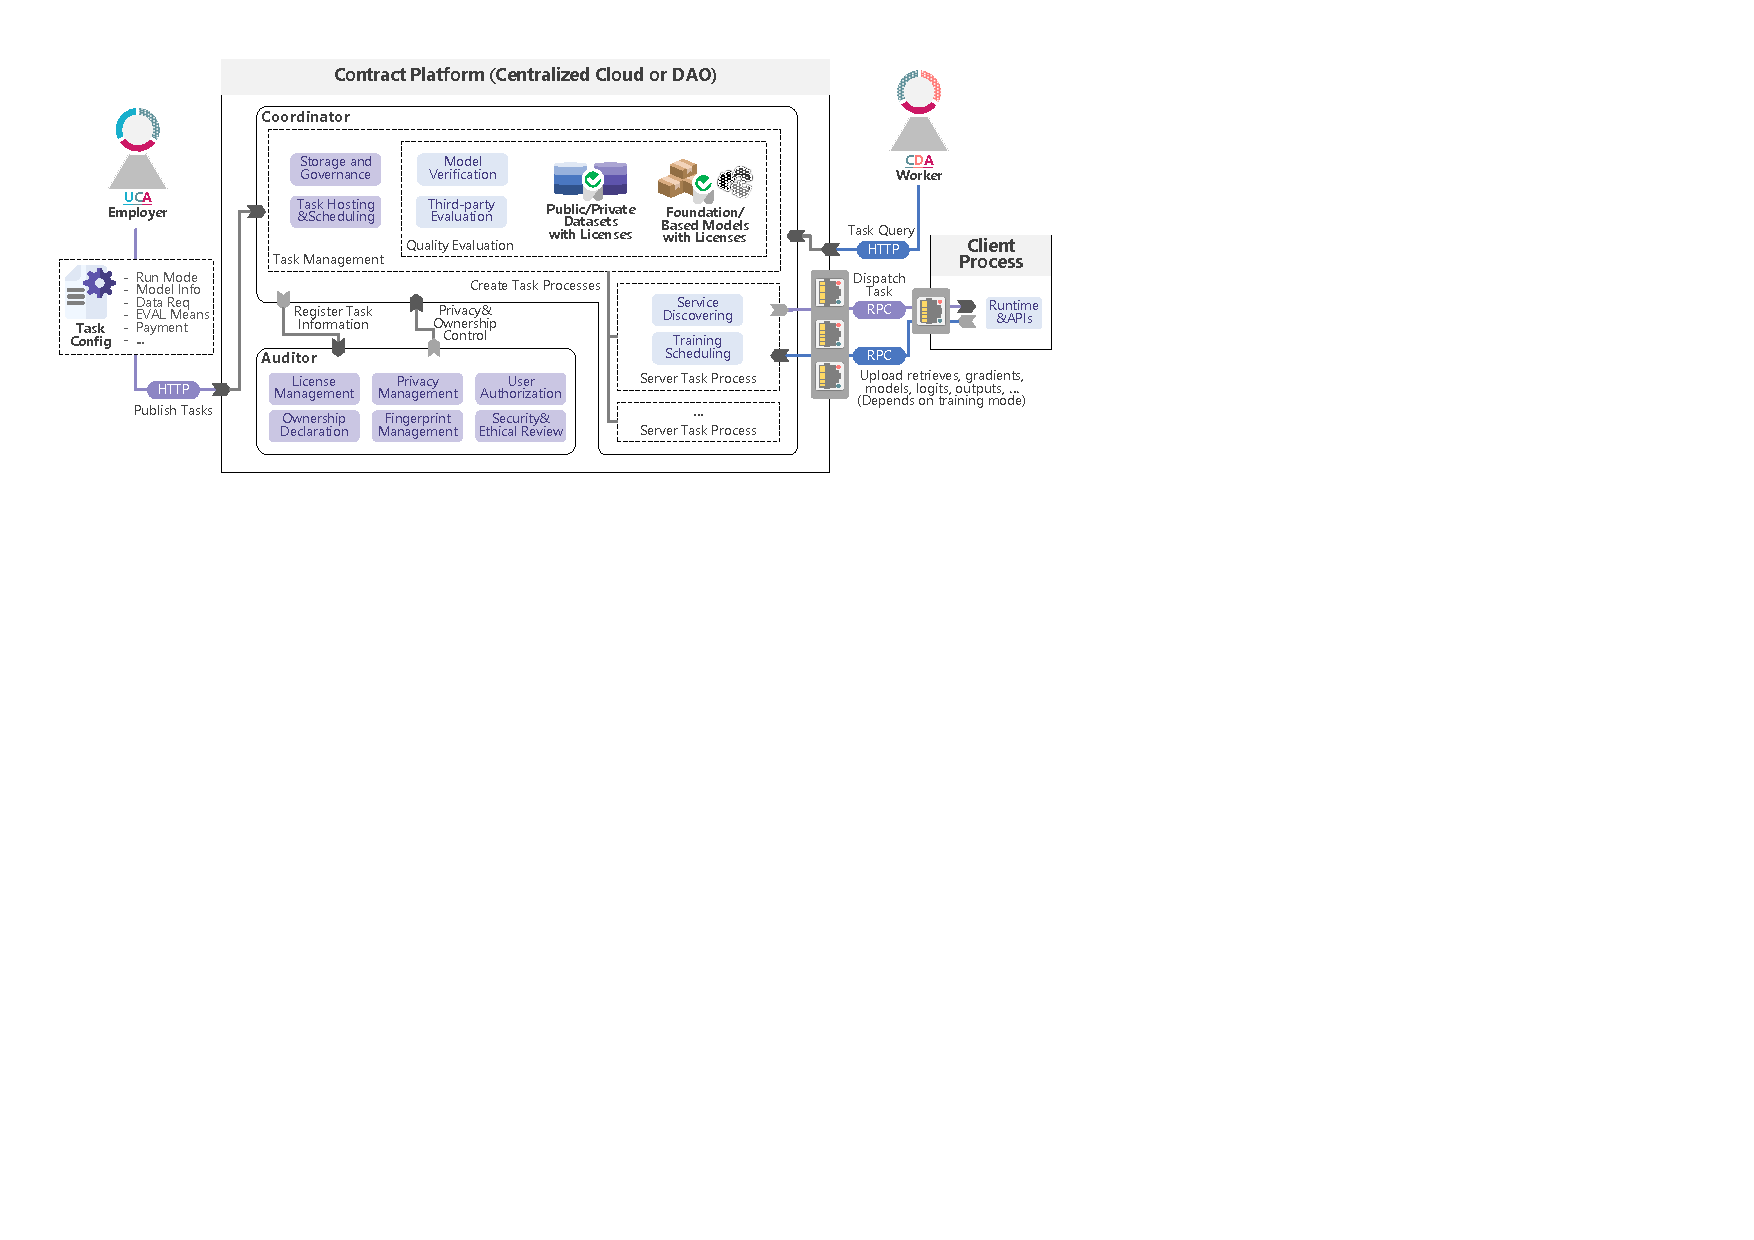
\includegraphics[width=\linewidth]{fig/contract_frame.pdf}
    \caption{An overview of contract-based FL systems. (U: model User, C: Coordinator, D: Data owner, A: Auditor)}
    \label{fig:contract}
\end{figure}

In short, contract-based FL retains all functionalities related to model training at the platform and only provides task publishing services to employers, who play the role of model training in traditional FL.
Furthermore, similar to model-reusing mechanisms (ref. \S\ref{sec:taxonomy}) that can be applied to query-based FL, our contract-based FL is not limited to an amalgamation-based collaborative training paradigm like FedAvg.
In fact, the contract platform is designed as a crowdsourcing platform among data miners for ML cooperation tasks, including distributed training, fine-tuning, and ensembling based on scratch or Foundation Models (FMs)~\cite{yuan2022decentralized}.
However, most current crowdsourcing platforms like Amazon Mechanical Turk and Appen\footnote{AMT: \url{https://www.mturk.com/}; Appen: \url{https://appen.com/crowd-2/}} primarily deal with human intelligence tasks such as data collection and annotation (aka. microtasks) rather than ML modeling tasks. 
It remains unexplored how to design and publish an ML task to seek crowd labor.
On the other hand, many studies~\cite{dias2022blocklearning, blythman2022decentralized, deng2021flex, guo2023blockchain, batool2022fl} and products~\cite{steeves2022incentivizing, ziller2021pysyft, mcconaghy2022ocean} emphasize monetizing ML activities through blockchain-based techniques and Decentralized Autonomous Organizations (DAOs). 
However, both monetization and decentralization are non-essential functions for our contract platforms\textsuperscript{\ddag{VI}}.
%, as we summarize and compare these works in Appendix~VI.


\begin{table*}[t]
    \centering
    \footnotesize
    \caption{Comparisons of typical model training frameworks with the intervention of a trustworthy platform. \colorbox{Employer!30}{\textasteriskcentered}, \colorbox{Platform!30}{\textasteriskcentered}, \colorbox{Worker!30}{\textasteriskcentered} indicate resources from \colorbox{Employer!30}{Employer}, \colorbox{Platform!30}{Platform}, and \colorbox{Worker!30}{Worker}, respectively. Resources in different color columns (e.g., \colorbox{Worker!30}{Data} in column \colorbox{Platform!30}{Platform}) represent transmission. $\bigstar$: Location of model training. \colorbox{Worker!30}{\textit{Resources}} received from other workers.}
    \label{tab:train}
    \begin{tabular}{|l|p{2.6cm}|p{4cm}|p{5cm}|}
    \hline
    & \multicolumn{1}{c|}{\cellcolor{Employer!30}{Employer}} & \multicolumn{1}{c|}{\cellcolor{Platform!30}{Platform}} & \multicolumn{1}{c|}{\cellcolor{Worker!30}{Worker}} \\ \hline
    
    Centralized ML & \colorbox{Employer!30}{Model} & \colorbox{Employer!30}{Model}\colorbox{Worker!30}{Data} $\bigstar$ & \colorbox{Worker!30}{Data} \\ \hline %Scratch

    FedAvg~\cite{mcmahan2017communication} & \colorbox{Employer!30}{Model} & \colorbox{Employer!30}{Model}\colorbox{Worker!30}{Gradient} & \colorbox{Employer!30}{Model}\colorbox{Worker!30}{Data} $\bigstar$ \\ \hline %Scratch

    DMoE~\cite{ryabinin2020towards} & \colorbox{Employer!30}{Gating NN}\colorbox{Employer!30}{Data} & \colorbox{Employer!30}{Gating NN}\colorbox{Employer!30}{Data}\colorbox{Worker!30}{Output} $\bigstar$ & \colorbox{Worker!30}{Model}\colorbox{Employer!30}{Data} $\bigstar$ \\ \hline %Scratch

    DeDES~\cite{wang2023data} & \colorbox{Worker!30}{Model Subset} & \colorbox{Worker!30}{Model} & \colorbox{Worker!30}{Model}\colorbox{Worker!30}{Data} $\bigstar$ \\ \hline %Scratch
    
    Borzunov \textit{et al.}~\cite{borzunov2022training} & \colorbox{Employer!30}{Model} & \colorbox{Employer!30}{Model}\colorbox{Platform!30}{Data}\colorbox{Worker!30}{Gradient} & \colorbox{Employer!30}{Model}\colorbox{Platform!30}{Data-Stream} $\bigstar$ \\ \hline %Scratch, DHT

    Moshpit SGD~\cite{ryabinin2021moshpit} & \colorbox{Employer!30}{Model}\colorbox{Employer!30}{Data} & \colorbox{Employer!30}{Model}\colorbox{Employer!30}{Data}\colorbox{Worker!30}{Gradient} & \colorbox{Employer!30}{Model}\colorbox{Employer!30}{Data-Loader} $\bigstar$ \\ \hline 

    VC-ASGD~\cite{atre2021distributed} & \colorbox{Employer!30}{Model}\colorbox{Employer!30}{Data} & \colorbox{Employer!30}{Model}\colorbox{Employer!30}{Data}\colorbox{Worker!30}{Gradient} & \colorbox{Employer!30}{Sub-model}\colorbox{Employer!30}{H-Data} $\bigstar$ \\ \hline

    SplitNN~\cite{vepakomma2019split} & \colorbox{Employer!30}{Model}\colorbox{Employer!30}{ID-Label} & \colorbox{Employer!30}{Model}\colorbox{Employer!30}{ID-Label}\colorbox{Worker!30}{Hidden} $\bigstar$ & \colorbox{Employer!30}{Sub-model}\colorbox{Worker!30}{V-Data}\colorbox{Platform!30}{Gradient} $\bigstar$ \\ \hline
    
    DT-FM~\cite{yuan2022decentralized} & \colorbox{Employer!30}{FM} & \colorbox{Employer!30}{FM}\colorbox{Platform!30}{Data} & \colorbox{Employer!30}{Sub-FM}\colorbox{Platform!30}{Micro-Batch}\colorbox{Worker!30}{\textit{Gradient}} $\bigstar$ \\ \hline

    FS-LLM~\cite{kuang2023federatedscope} & \colorbox{Employer!30}{FM} & \colorbox{Employer!30}{FM}\colorbox{Worker!30}{Adapter} & \colorbox{Employer!30}{FM}\colorbox{Worker!30}{Data} $\bigstar$ \\ \hline

    FedKSeed~\cite{qin2023federated} & \colorbox{Employer!30}{FM} & \colorbox{Employer!30}{FM}\colorbox{Platform!30}{Seed}\colorbox{Worker!30}{Scaler Gradient} & \colorbox{Employer!30}{FM}\colorbox{Platform!30}{Seed}\colorbox{Worker!30}{Data} $\bigstar$ \\ \hline

    Berdoz \textit{et al.}~\cite{berdoz2022scalable} & \colorbox{Employer!30}{Class} & \colorbox{Employer!30}{Class}\colorbox{Platform!30}{NN Structure}\colorbox{Worker!30}{Hidden} & \colorbox{Platform!30}{NN Structure}\colorbox{Worker!30}{Data}\colorbox{Platform!30}{Hidden AVG} $\bigstar$ \\ \hline

    CCL~\cite{aketi2024cross} & \colorbox{Employer!30}{Class} & \colorbox{Employer!30}{Class} & \colorbox{Worker!30}{Data}\colorbox{Worker!30}{\textit{Model}}\colorbox{Worker!30}{\textit{Hidden AVG}} $\bigstar$ \\ \hline

    FedProto~\cite{tan2022fedproto, michieli2021prototype} & \colorbox{Employer!30}{Class} & \colorbox{Employer!30}{Class}\colorbox{Worker!30}{Hidden} & \colorbox{Worker!30}{Data}\colorbox{Worker!30}{Model}\colorbox{Platform!30}{Hidden AVG} $\bigstar$ \\ \hline   

    Ocean~\cite{mcconaghy2022ocean} & \colorbox{Employer!30}{Model}\colorbox{Worker!30}{Output} & \colorbox{Worker!30}{Metadata} & \colorbox{Worker!30}{Metadata}\colorbox{Employer!30}{Model}\colorbox{Worker!30}{Data} $\bigstar$ \\ \hline

    \end{tabular}
\end{table*}

\subsection{How to Design ML Microtasks}
\label{sec:how2design}
When we come to the scenario of contract-based FL, we first need to define how to design ML microtasks for crowd workers. 
Unfortunately, previous collaborative ML studies~\cite{li2021survey, nguyen2021federated} rarely discuss this question because they default to assuming that all employers or workers have the same resource type to fit into their modeling frameworks.
On the contrary, in contract-based FL, we leave the freedom of design microtasks and choosing modeling method to the employers.

%The answer to this question depends on what resources the employers have and what tasks the workers can perform.
The answer depends on what resources the employers have and what tasks the workers can perform.
For example, in horizontal FL, the server should provide an initial model, and clients should have training data under the same feature space and provide computational power. However, in vertical FL, the clients should have training data under the same sample space (i.e., ID space). 
This difference determines which modeling framework employers can adopt. 
Following this idea, we provide comparisons of typical FL, distributed ML, and blockchain-based modeling frameworks in TABLE~\ref{tab:train}.
For simplicity, we introduce the \textbf{Platform} between Employer and Worker in some frameworks to make it adaptable for contract-based FL. 
You can quickly restore the original structure by merging Employer and Platform columns.
To represent the transmission of resources, we mark resources provided by each group of entities with different colors.
The computational resource used for training is marked with $\bigstar$.
By this way, we can conveniently find the feasible and privacy-preserving modeling frameworks for collaborative learning. 
Here, we briefly introduce these frameworks group by scenarios\footnote{From the viewpoint of Employers.}.

\subsubsection{Train from scratch with workers' private data}
There are four frameworks that support this scenario. 
The first is \textbf{Centralized ML}, which requires workers to upload their data to a cloud platform for modeling. However, this approach is not feasible for FL scenarios due to privacy concerns. 
The second is \textbf{FedAvg}~\cite{mcmahan2017communication}, which requires workers to upload computed gradients upon the scratch model and their private data (horizontally split). Computing resources need to be provided by workers as well.
The third is \textbf{SplitNN}~\cite{vepakomma2019split}, where each worker trains the cut layers of the model using their vertically split data. 
The hidden representations from these layers are uploaded to the platform for the training of the remaining layers.
The last and distinctive is a Web3 system named \textbf{Ocean}~\cite{mcconaghy2022ocean}.
It enables workers to upload only the metadata of their local dataset to a blockchain-based platform to attract buyers. 
Interested buyers then need to purchase datatokens to access the local dataset and deploy their modeling algorithm. 
To ensure the privacy and IP security of workers, only trusted algorithms are allowed, and only model predictions will be sent to buyers.

\subsubsection{Ensemble workers' private model} %优点:支持模型异构
As we presented in \S\ref{sec:taxonomy}, ensembling is an effective method to integrate knowledge, and the distributed version is proposed by \textbf{DMoE}~\cite{ryabinin2020towards}. 
It employs a Distributed Hash Table (DHT) to store metadata and worker statuses, constructing a decentralized expert network. 
To make inferences using this network, each model user must train a local gating network to select a subset of experts tailored to their input.
No additional training required, Wang \textit{et al.} purposed \textbf{DeDES}~\cite{wang2023data}, which selects a diverse subsect of weak models from population and make inference by voting. 
The unique advantage of ensembling lies in its inherent support for model heterogeneity, and its integration is extensible. 
This capability enables the establishment of a cooperative network while maintaining flexibility and availability.

\subsubsection{Train from fundation model}
Foundation models, trained on larger-scale data with robust generalization abilities across various downstream tasks, serve as a solid foundation for collaborative training. 
Yuan \textit{et al.} proposed \textbf{DT-FM}~\cite{yuan2022decentralized} to establish an effective geo-distributed learning system across 8 regions for training the language model GPT-3.
Similarly, Borzunov \textit{et al.}\cite{borzunov2022training} recruited volunteer nodes to train a transformer model over the Internet. 
To enhance system robustness, \textbf{Moshpit SGD}~\cite{ryabinin2021moshpit} divides worker nodes into small, independent groups to ensure that all-reduce is not affected by the failure of a single participant.
Additionally, \textbf{VC-ASGD}\cite{atre2021distributed} divides the deep learning training job into asynchronous parameter update subtasks to improve scalability.
In these cases, employers are required to supply the initial model and training data needed to launch training subtasks. 
This training paradigm is particularly suitable for worker nodes that possess computational and communication resources but lack their own training data.

Instead of initiating training from scratch and consuming substantial computational resources, we can also collaboratively adapt these foundation models to specific local tasks based on relatively restricted hardware and data size through fine-tuning.
Recently, Woisetschl{\"a}ger \textit{et al.}~\cite{woisetschlager2023federated} have explored the opportunity to fine-tune large language models, such as FLAN-T5, by edge devices.
Simultaneously, \textbf{FS-LLM}~\cite{kuang2023federatedscope} employs Parameter-Efficient Fine-Tuning (PEFT) methods for federated fine-tuning of LLaMA-7B, minimizing communication and computation costs.
\textbf{FATE-LLM}~\cite{fan2023fate} offers a solution called FedHeteroLLM, leveraging KD to train a mentee model from its local pre-trained LLM for federated aggregation.
To alleviate the computational burden associated with backpropagation-based optimization methods, \textbf{FedKSeed}~\cite{qin2023federated} employs zeroth-order optimization (ZOO). 
Only seed and scalar gradients need to be transmitted for federated fine-tuning.

\subsubsection{Representations Sharing}
Another popular scheme for organizing ML microtasks involves sharing the learned representations of workers. 
For instance, the use of class-conditional average of last hidden layer activations (aka. Prototypes) can enhance class discrimination across different clients~\cite{aketi2024cross, tan2022fedproto, michieli2021prototype, berdoz2022scalable}.
To configure the microtasks, employers only need to set the target class, after which the platform can collect and distribute per-class prototypes among workers.
With no central server required, \textbf{CCL}~\cite{aketi2024cross} presents a decentralized learning approach based on cross-workers prototypes sharing.
%However, the choosing between central solution and decentral solution is depends on what kind of infrastructure are perfered.
%For example, we can decentralized the store of local mode by IPFS~\cite{benet2014ipfs} protocol

\subsection{Limitations of Contract-based FL}
\label{sec:limitations_cbfl}
In contract-based FL systems, employers can publish their personalized ML crowdsourcing tasks, considering both their local resources and the resources of the target clients. 
However, to meet the flexibility requirements of widely supporting training methods, the contract platform should offer highly compatible APIs that can integrate various distributed training frameworks. 
Additionally, it needs to provide comprehensive audit against malicious users and plagiarism, significantly increasing the complexity compared to traditional FL and query-based FL.
Meanwhile, to establish confidence among users, a fair and consensual third-party model evaluation mechanism should be established, which, however, is almost unexplored in the current academic studies.



\section{Conclusion}
\label{sec:conclusion}
Traditional federated learning systems with a server-dominated cooperation framework suppress the enthusiasm of participants and limit the further extension of such collaboration. 
To explore the opportunity to establish a more open and reciprocal cooperation platform, we investigate current progress in federated learning, decentralized machine learning, and model reusing systems. 
In this way, we depict two rough sketches of open federated learning platforms: query-based federated learning paltform and contract-based federated learning paltform. 
Based on these two proposed platforms, we survey their possible supported techniques and their related legal issues, including ML licensing and copyrightability. 
We believe this survey can encourage a rethinking of current collaborative ML systems design and lead to the pervasive availability of AI for everyone.


%Therefore, we don't delve into this topic in this survey.

% 目标:1)保护任务发布方的利益和隐私;2)保护数据所有者的利益和隐私;3)遏制侵权行为

% 如何衡量模型质量:1)第三方evaluation

% 如果不采用pipeline的方式训练,如何拆分训练任务?

% 如何发现可用的FL节点
% 几种训练组织方式
